In order to assess how the identified models generalize into a situation with wind, predictions have been conducted for an idealized wind state. The idealized wind state is a very simplified hydrodynamic condition where the models have a drift angle, but no yaw rate, or rudder angle. This is meant to represent a state where the ship is experiencing a static drift angle for a long time -- induced by a side wind force.
The prediction results for the idealized wind condition are shown in \autoref{fig:result_wind_state}. The sway force $Y_D$ of the Physics informed model is very similar to the Reference model; For the Abkowitz model the sway force seems to be too large. The yawing moment $N_D$ is under predicted by both models, but the difference is much larger for the Abkowitz model. 
This is because most of the yawing moment is denoted to the yaw rate coefficients (as previously stated in \autoref{sec:result_MDL}) -- which are not activated in the wind state. 
The Physics informed model seems to have a split between the yaw rate and drift angle dependent coefficients that is much more similar to the more physically correct Reference model.
\label{sec:wind_state}
\begin{figure}[h!]
    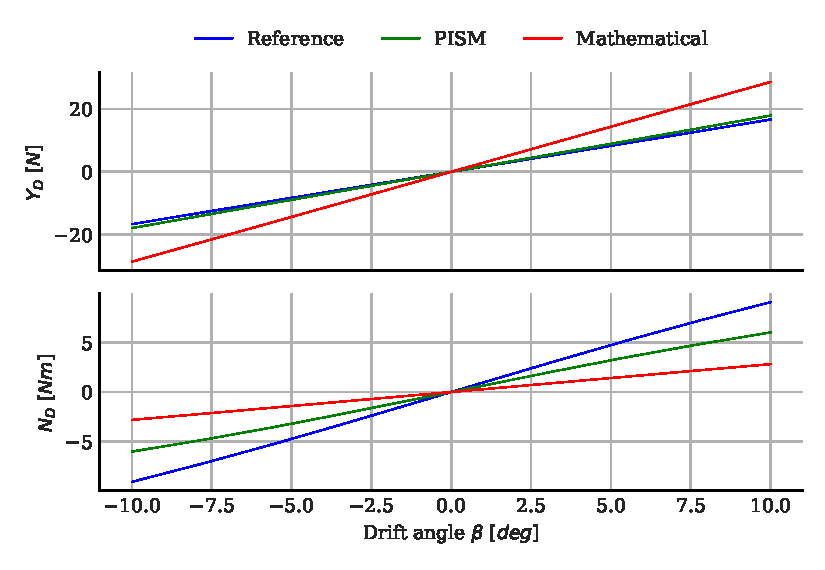
\includegraphics[width=\columnwidth]{figures/result_wind_state.forces.pdf}
    \caption{Total sway force and yawing moment from the models at various drift angles.}
    \label{fig:result_wind_state}
\end{figure}